\documentclass[10pt]{beamer}
\usepackage[english]{babel}
\usepackage[utf8]{inputenc}
\usepackage[T1]{fontenc}
\usepackage{helvet}
\usepackage{multicol}
%-------------------------------------------------------
% INFORMATION IN THE TITLE PAGE
%-------------------------------------------------------

\newcommand{\cstitle}{\textbf{Data bases}}
\subtitle[]{UMTG: a toolset to automatically generate system test cases from use case specifications}
\newcommand{\cscourseCode}{Data bases}
\newcommand{\csauthor}{MSc. Vicente Machaca Arceda}
\institute[UNSA]{Universidad Nacional de San Agustín}
\newcommand{\csemail}{vmachacaa@unsa.edu.pe}
\newcommand{\instituteabr}{UNSA}
\newcommand{\nameUp}{}
\date{2021}
\title[\cscourseCode]{\cstitle}
\author{\csauthor}
%%%%%%%%%%%%%%%%%

%-------------------------------------------------------
% CHOOSE THE THEME
%-------------------------------------------------------
\def\mycmd{0} % CS THEME
\def\mycmd{1} % MYTHEME
%-------------------------------------------------------

\if\mycmd1
	\usetheme[]{Feather}
	\newcommand{\chref}[2]{\href{#1}{{\usebeamercolor[bg]{Feather}#2}}}
\else
	\usepackage{csformat}
	\newcommand{\chref}[3][blue]{\href{#2}{\color{#1}{#3}}}%
\fi

\newcommand{\1}{
        	\setbeamertemplate{background}{
        		
\includegraphics[width=\paperwidth,height=\paperheight]{img/1}
        		\tikz[overlay] \fill[fill opacity=0.75,fill=white] (0,0) rectangle (-\paperwidth,\paperheight);
        	}
}



%-------------------------------------------------------
% THE BODY OF THE PRESENTATION
%-------------------------------------------------------

\begin{document}


%\AtBeginSubsection[]
%{
%    \begin{frame}
%        \frametitle{Overview}
%        \tableofcontents[currentsubsection]
%    \end{frame}
%}


%-------------------------------------------------------
% THE TITLEPAGE
%-------------------------------------------------------

\if\mycmd1 % MY THEME
	\1{
	\begin{frame}[plain,noframenumbering] 
		\titlepage 
	\end{frame}}

\else % CS THEME
	\maketitle
\fi


%-------------------------------------------------------
%-------------------------------------------------------
\begin{frame}{Content}
	\tableofcontents
\end{frame}
%-------------------------------------------------------
%-------------------------------------------------------


%%%%%%%%%%%%%%%%%%%%%%%%%%%%%%%%%%%%%%%%%%%%%%%%%%%%%%%%%%%%%%%%%%%%%%%%%%%%%%%%%%%%%%%%%%%%%%%%%%%%%%%%%%%%%%%%
%%%%%%%%%%%%%%%%%%%%%%%%%%%%%%%%%%%%%%%%%%%%%%%%%%%%%%%%%%%%%%%%%%%%%%%%%%%%%%%%%%%%%%%%%%%%%%%%%%%%%%%%%%%%%%%%
%%%%%%%%%%%%%%%%%%%%%%%%%%%%%%%%%%%%%%%%%%%%%%%%%%%%%%%%%%%%%%%%%%%%%%%%%%%%%%%%%%%%%%%%%%%%%%%%%%%%%%%%%%%%%%%%
\section{UMTG}
%%%%%%%%%%%%%%%%%%%%%%%%%%%%%%%%%%%%%%%%%%%%%%%%%%%%%%%%%%%%%%%%%%%%%%%%%%%%%%%%%%%%%%%%%%%%%%%%%%%%%%%%%%%%%%%%
%%%%%%%%%%%%%%%%%%%%%%%%%%%%%%%%%%%%%%%%%%%%%%%%%%%%%%%%%%%%%%%%%%%%%%%%%%%%%%%%%%%%%%%%%%%%%%%%%%%%%%%%%%%%%%%%
%%%%%%%%%%%%%%%%%%%%%%%%%%%%%%%%%%%%%%%%%%%%%%%%%%%%%%%%%%%%%%%%%%%%%%%%%%%%%%%%%%%%%%%%%%%%%%%%%%%%%%%%%%%%%%%%

%%%%%%%%%%%%%%%%%%%%%%%%%%%%%%%%%%%%%%%%%%%%%%%%%%%%%%%%%%%%%%%%%%%%%%%%%%%%%%%%%%%%%%%%%%%%%%%%%%%%%%%%%%%%%%%%
%%%%%%%%%%%%%%%%%%%%%%%%%%%%%%%%%%%%%%%%%%%%%%%%%%%%%%%%%%%%%%%%%%%%%%%%%%%%%%%%%%%%%%%%%%%%%%%%%%%%%%%%%%%%%%%%
%%%%%%%%%%%%%%%%%%%%%%%%%%%%%%%%%%%%%%%%%%%%%%%%%%%%%%%%%%%%%%%%%%%%%%%%%%%%%%%%%%%%%%%%%%%%%%%%%%%%%%%%%%%%%%%%
\subsection{Definition}
%%%%%%%%%%%%%%%%%%%%%%%%%%%%%%%%%%%%%%%%%%%%%%%%%%%%%%%%%%%%%%%%%%%%%%%%%%%%%%%%%%%%%%%%%%%%%%%%%%%%%%%%%%%%%%%%
%%%%%%%%%%%%%%%%%%%%%%%%%%%%%%%%%%%%%%%%%%%%%%%%%%%%%%%%%%%%%%%%%%%%%%%%%%%%%%%%%%%%%%%%%%%%%%%%%%%%%%%%%%%%%%%%
%%%%%%%%%%%%%%%%%%%%%%%%%%%%%%%%%%%%%%%%%%%%%%%%%%%%%%%%%%%%%%%%%%%%%%%%%%%%%%%%%%%%%%%%%%%%%%%%%%%%%%%%%%%%%%%%

%-------------------------------------------------------
%-------------------------------------------------------
\begin{frame}{UMTG}{}	
	\begin{block}{}
		UMTG, a toolset that generates	executable system test cases by exploiting the behavioural	information implicitly described in use case specifications \cite{wang2015umtg}.
	\end{block}	

	\begin{block}{}
		UMTG generates OCL constraints for:
		\begin{itemize}
			\item Use case preconditions.
			\item Postconditions.
			\item Conditional steps.
		\end{itemize}.
	\end{block}	

\end{frame}
%-------------------------------------------------------
%-------------------------------------------------------

%-------------------------------------------------------
%-------------------------------------------------------
\begin{frame}{UMTG}{OCL constraints}	
\begin{table}
	\caption{Examples of OCL constraints.}
	\begin{tabular}{|p{4cm}|p{5.8cm}|}
		\hline 
		\textbf{Constraint} & \textbf{OCL Equivalent}   \\	\hline 
		The age of a person is not negative & \textbf{context} Person \textbf{inv}: self.age >=0 \\ \hline
		
		A Person has 2 parents at max & \textbf{context} Person \textbf{inv}: self.parents->size()<=2 \\ \hline	
		
		%There's at least one Person which owns a car & 	\textbf{context} Person \textbf{inv}: Person.allInstances()->exists(p | p.cars->size() > 0) \\ \hline
		
		The system sets the occupancy status to empty & \textbf{BodySense}.allinstances()->forAll( i|i.occupancyStatus = \textbf{Occupancy::Empty} ) \\ \hline
		
	\end{tabular}
\end{table}	
\end{frame}
%-------------------------------------------------------
%-------------------------------------------------------

%-------------------------------------------------------
%-------------------------------------------------------
\begin{frame}{UMTG}{}	
	\begin{figure}
		\centering
		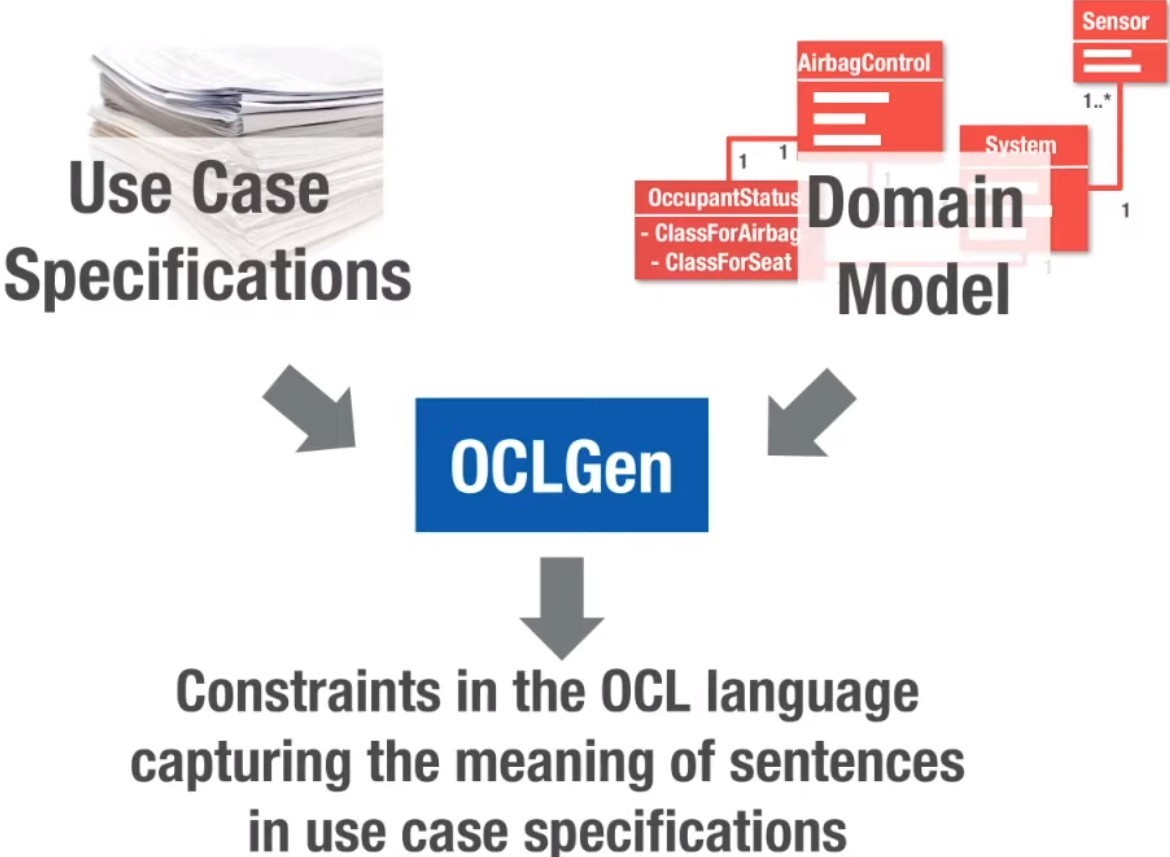
\includegraphics[width=0.7\textwidth]{img/umtg/umtg}
	\end{figure}	
\end{frame}
%-------------------------------------------------------
%-------------------------------------------------------




%%%%%%%%%%%%%%%%%%%%%%%%%%%%%%%%%%%%%%%%%%%%%%%%%%%%%%%%%%%%%%%%%%%%%%%%%%%%%%%%%%%%%%%%%%%%%%%%%%%%%%%%%%%%%%%%
%%%%%%%%%%%%%%%%%%%%%%%%%%%%%%%%%%%%%%%%%%%%%%%%%%%%%%%%%%%%%%%%%%%%%%%%%%%%%%%%%%%%%%%%%%%%%%%%%%%%%%%%%%%%%%%%
%%%%%%%%%%%%%%%%%%%%%%%%%%%%%%%%%%%%%%%%%%%%%%%%%%%%%%%%%%%%%%%%%%%%%%%%%%%%%%%%%%%%%%%%%%%%%%%%%%%%%%%%%%%%%%%%
\subsection{Workflow}
%%%%%%%%%%%%%%%%%%%%%%%%%%%%%%%%%%%%%%%%%%%%%%%%%%%%%%%%%%%%%%%%%%%%%%%%%%%%%%%%%%%%%%%%%%%%%%%%%%%%%%%%%%%%%%%%
%%%%%%%%%%%%%%%%%%%%%%%%%%%%%%%%%%%%%%%%%%%%%%%%%%%%%%%%%%%%%%%%%%%%%%%%%%%%%%%%%%%%%%%%%%%%%%%%%%%%%%%%%%%%%%%%
%%%%%%%%%%%%%%%%%%%%%%%%%%%%%%%%%%%%%%%%%%%%%%%%%%%%%%%%%%%%%%%%%%%%%%%%%%%%%%%%%%%%%%%%%%%%%%%%%%%%%%%%%%%%%%%%



%-------------------------------------------------------
%-------------------------------------------------------
\begin{frame}{Workflow}{}	
	\begin{figure}
		\centering
		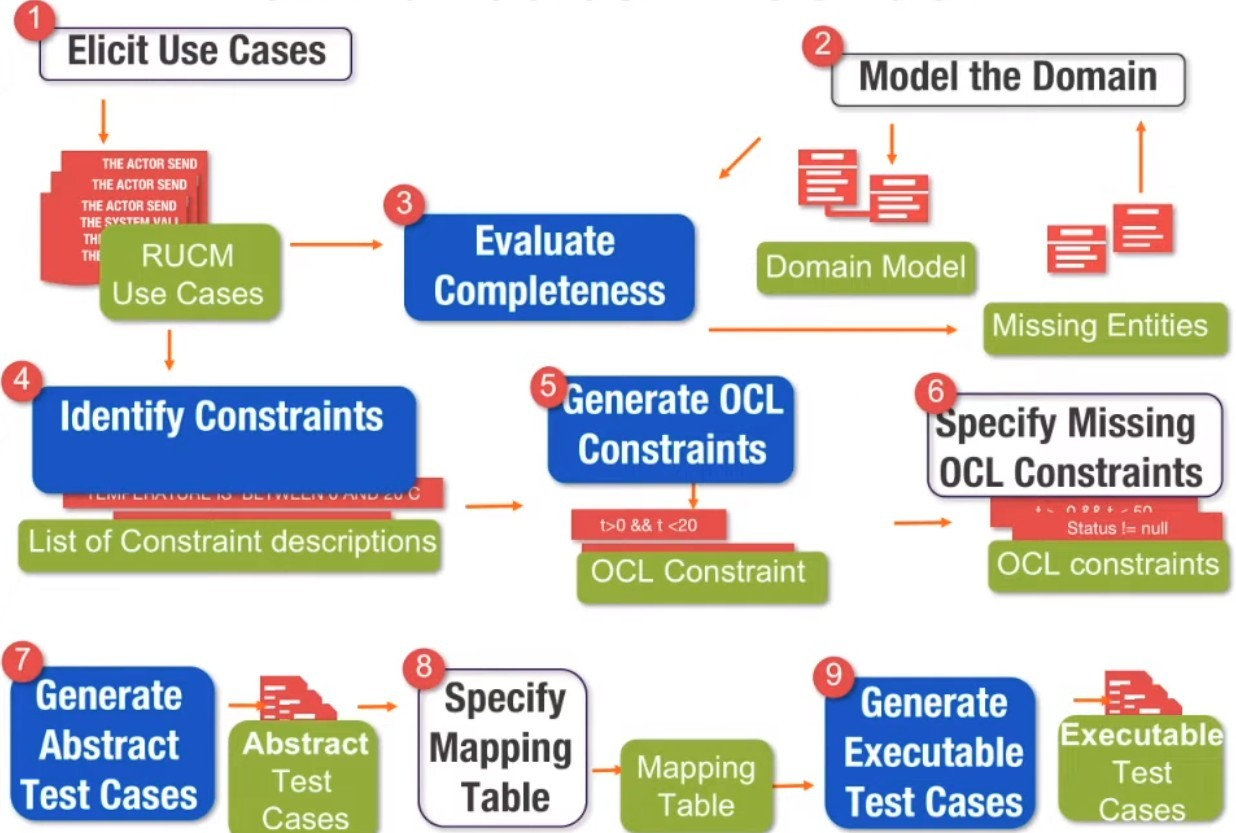
\includegraphics[width=0.9\textwidth]{img/umtg/arch}
	\end{figure}	
\end{frame}
%-------------------------------------------------------
%-------------------------------------------------------


%-------------------------------------------------------
%-------------------------------------------------------
\begin{frame}{Workflow}{RUCM use cases}	
	\begin{figure}
		\centering
		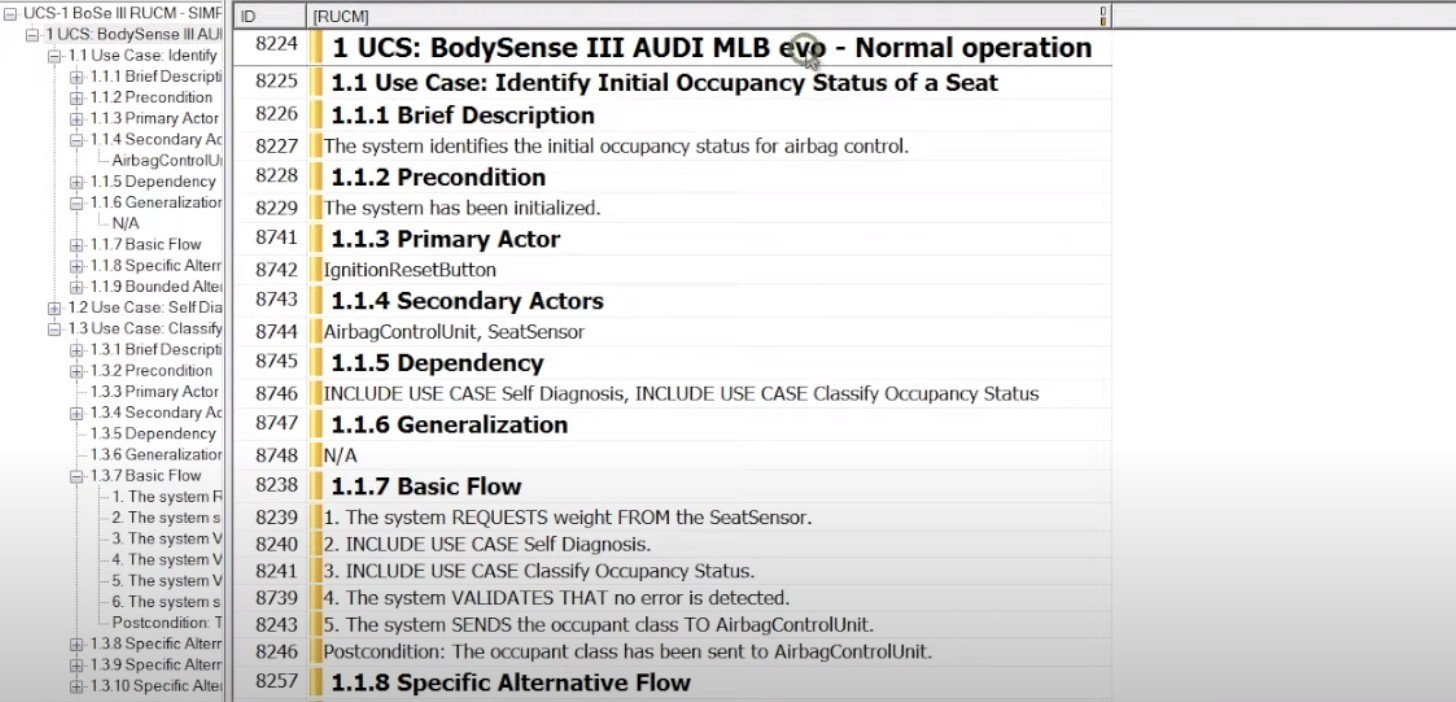
\includegraphics[width=\textwidth]{img/umtg/rucm}
		\caption{RUCM Use Case Specification in IBM DOORS.}
	\end{figure}	
\end{frame}
%-------------------------------------------------------
%-------------------------------------------------------

%-------------------------------------------------------
%-------------------------------------------------------
\begin{frame}{Workflow}{OCL constraints}	
	\begin{figure}
		\centering
		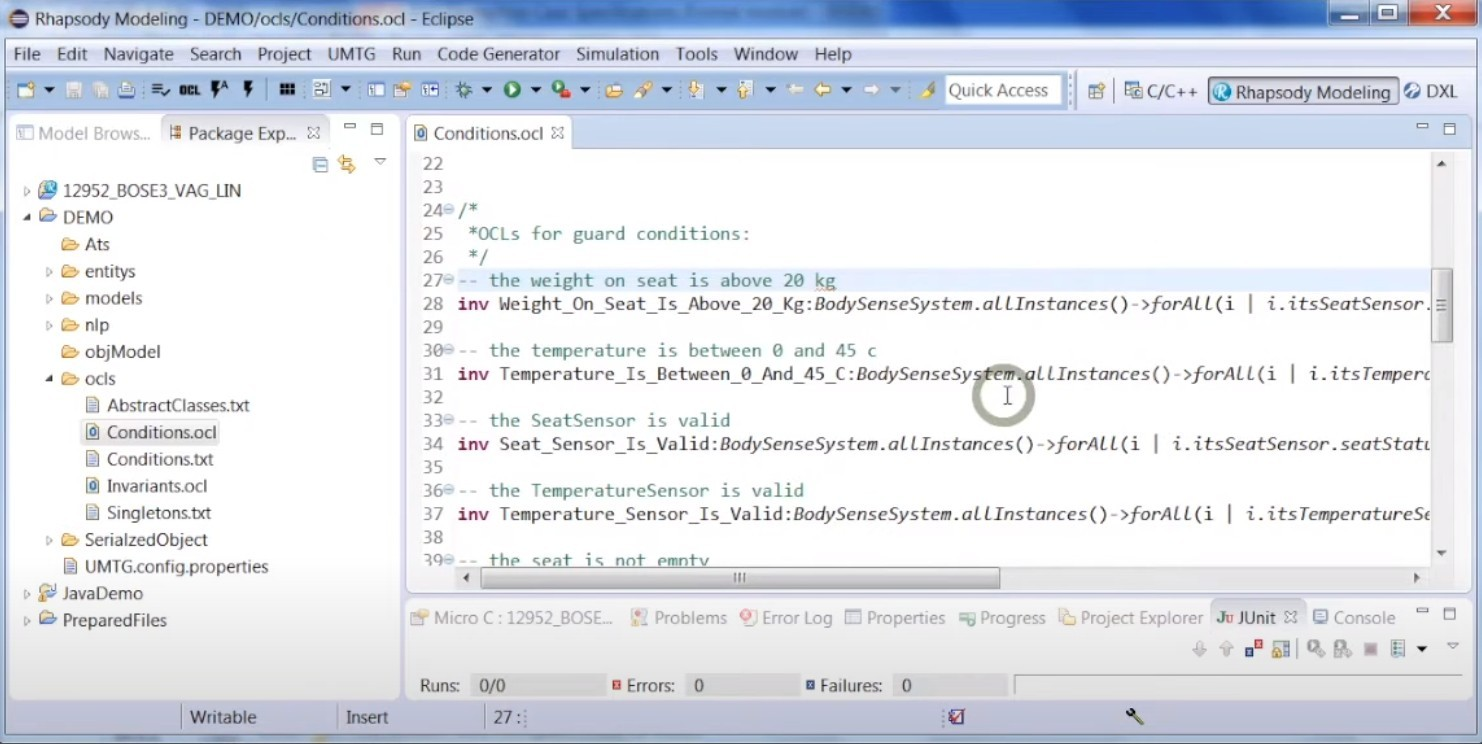
\includegraphics[width=\textwidth]{img/umtg/ocl}
		\caption{OCL constraints generated by UMTG.}
	\end{figure}	
\end{frame}
%-------------------------------------------------------
%-------------------------------------------------------

%-------------------------------------------------------
%-------------------------------------------------------
\begin{frame}{Workflow}{Abstract test cases}	
	\begin{figure}
		\centering
		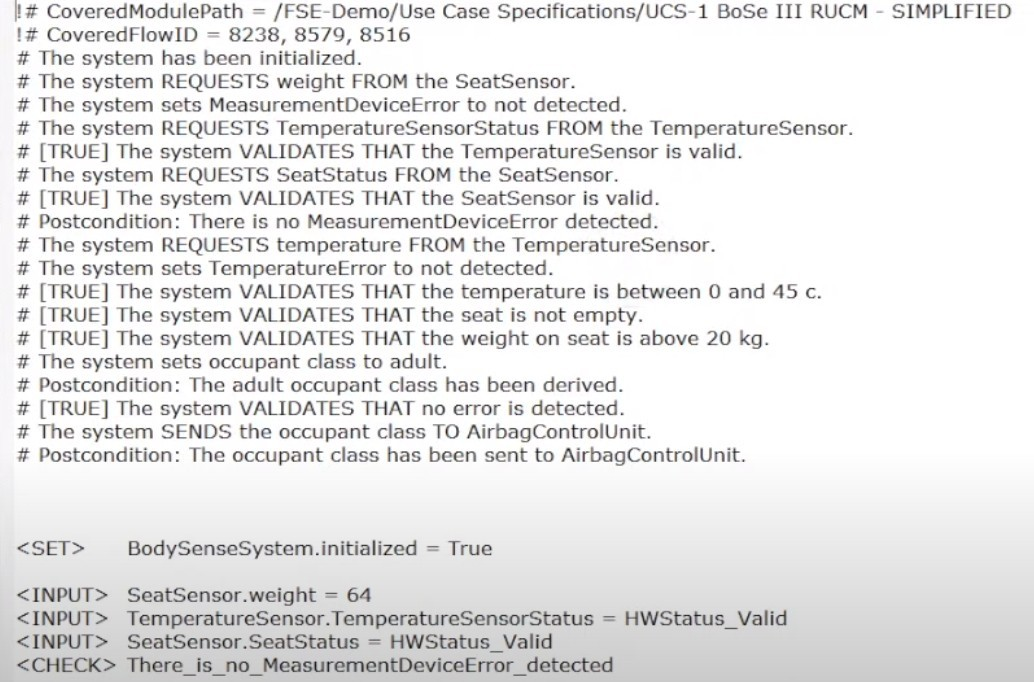
\includegraphics[width=0.9\textwidth]{img/umtg/atc}
		\caption{Abstract test cases.}
	\end{figure}	
\end{frame}
%-------------------------------------------------------
%-------------------------------------------------------

%-------------------------------------------------------
%-------------------------------------------------------
\begin{frame}{Workflow}{Mapping table}	
	\begin{figure}
		\centering
		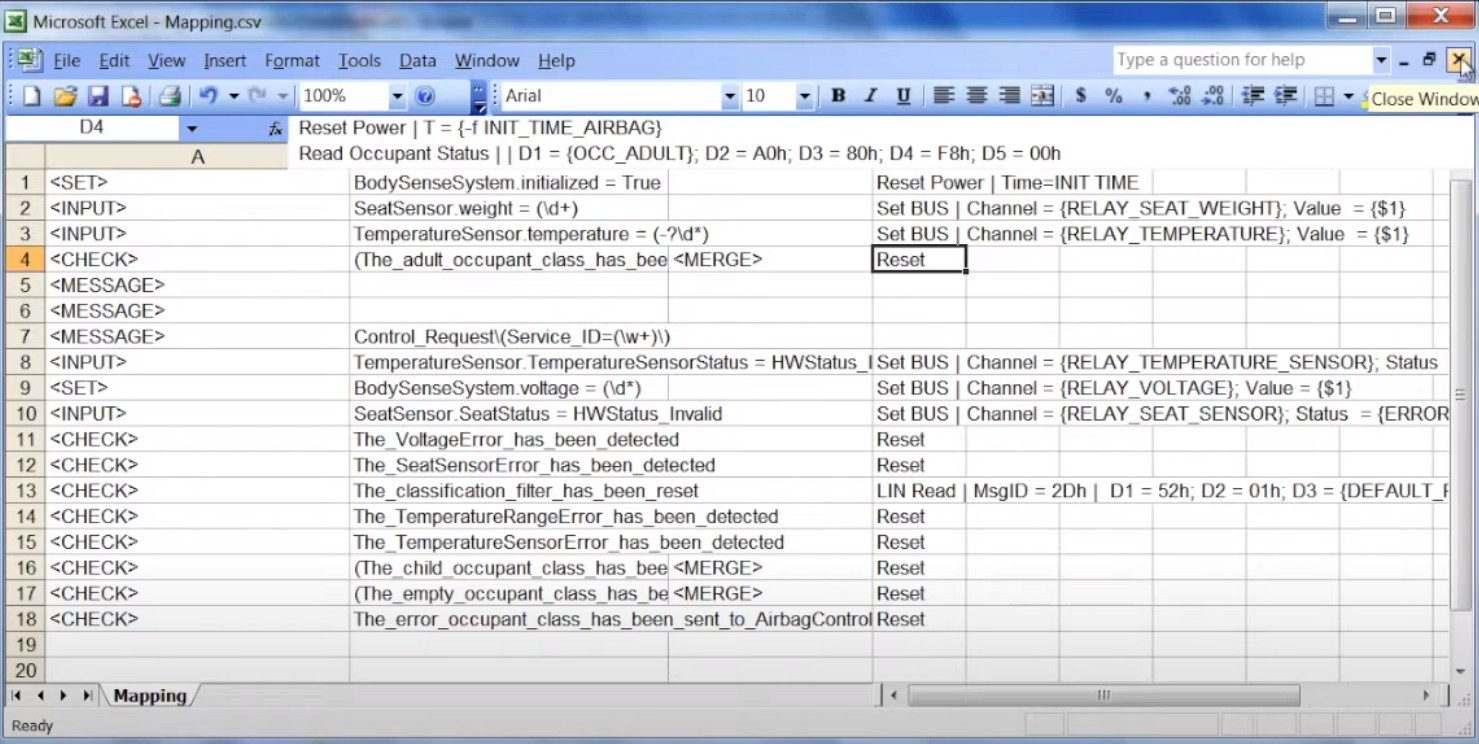
\includegraphics[width=0.9\textwidth]{img/umtg/map}
		\caption{Mapping table.}
	\end{figure}	
\end{frame}
%-------------------------------------------------------
%-------------------------------------------------------

%-------------------------------------------------------
%-------------------------------------------------------
\begin{frame}{Workflow}{Test case}	
	\begin{figure}
		\centering
		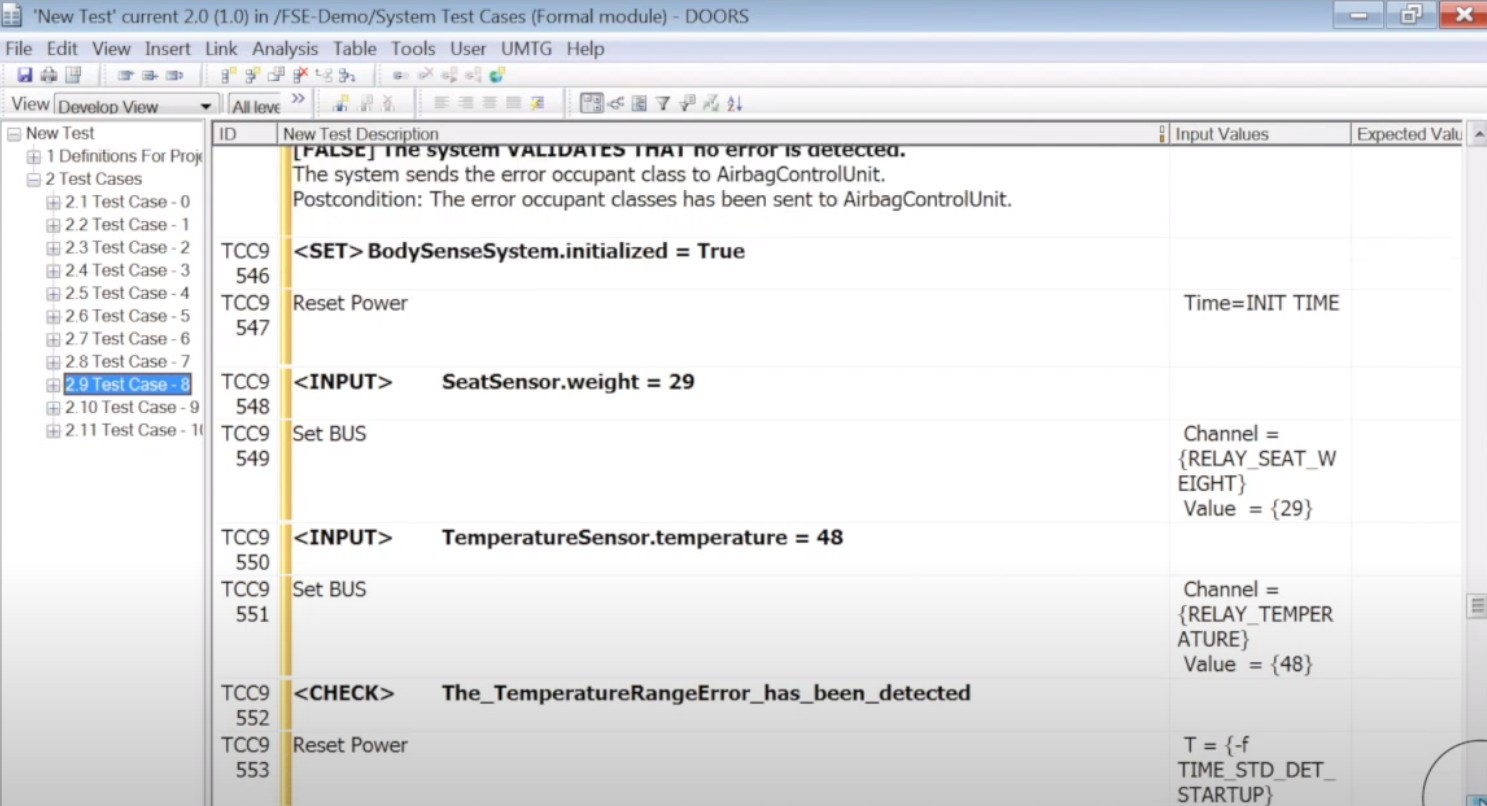
\includegraphics[width=0.9\textwidth]{img/umtg/testcase}
		\caption{Test case.}
	\end{figure}	
\end{frame}
%-------------------------------------------------------
%-------------------------------------------------------


%-------------------------------------------------------
%-------------------------------------------------------
\begin{frame}[allowframebreaks]
	\frametitle{References}
	%\bibliographystyle{amsalpha}
	\bibliographystyle{IEEEtran}
	\bibliography{bibliography.bib}
\end{frame}
%-------------------------------------------------------
%-------------------------------------------------------


%-------------------------------------------------------
%-------------------------------------------------------
\if\mycmd1 % MY THEME
\1{
	{\1
		\begin{frame}[plain,noframenumbering]
			%\finalpage{Thank you}
			\begin{figure}[]
				\centering
				
\includegraphics[width=\textwidth,height=0.7\textheight,keepaspectratio]{img/question.png}
				%\label{img:mot2}
				%\caption{Image example in 2 gray levels.}
			\end{figure}
	\end{frame}}
	\else % CS THEME
	\begin{frame}{Questions?}
		\begin{figure}[]
			\centering
			
\includegraphics[width=\textwidth,height=0.7\textheight,keepaspectratio]{img/question.png}
			%\label{img:mot2}
			%\caption{Image example in 2 gray levels.}
		\end{figure}
		
	\end{frame}
	\fi
	%-------------------------------------------------------
	%-------------------------------------------------------
	

\end{document}